\documentclass{article}
\usepackage[utf8]{inputenc}
\usepackage[a4paper,
            tmargin=2cm,
            bmargin=2cm,
            lmargin=2cm,
            rmargin=2cm,
            bindingoffset=0cm]{geometry}

\usepackage{lmodern}
\usepackage[T1]{polski}
\usepackage[utf8]{inputenc}
\usepackage{tocloft}
\usepackage{hyperref}
\usepackage{amsmath}
\usepackage{listings}
\usepackage{graphicx}
\usepackage{subfig}
\usepackage{float}
\usepackage{booktabs}
\usepackage{algpseudocode}

\hypersetup{
    colorlinks,
    citecolor=black,
    filecolor=black,
    linkcolor=black,
    urlcolor=black
}

\title {
        Algorytmy Macierzowe \\
        Sprawozdanie 5 \\
        Reordering w celu optymalizacji kompresji macierzy

}

\author{Przemek Węglik \\ Szymon Paszkiewicz}

\date{\today}

\begin{document}

\maketitle

\newpage

\section{Fragmenty kodu}

Funkcja realizująca minimum degree reordering:

\begin{lstlisting}[language=Python]
    def minimum_degree_transformation(input_matrix: np.ndarray) -> np.ndarray:
    E = list(zip(*np.nonzero(input_matrix)))
    graph = [{i} for i in range(input_matrix.shape[0])]
    for e in E:
        graph[e[0]].add(e[1])
        graph[e[1]].add(e[0])

    order = []
    for _ in range(len(graph)):
        v = -1
        min_deg = len(input_matrix)

        for j, s in enumerate(graph):
            if len(s) != 0 and len(s) < min_deg:
                v = j
                min_deg = len(s)

        order.append(v)
        for s in graph:
            if v in s:
                s.remove(v)
        graph[v].clear()

    inverted = [None for _ in range(len(order))]
    for i, o in enumerate(order):
        inverted[o] = i

    result = np.zeros(input_matrix.shape)
    for coord in E:
        result[inverted[coord[0]]][inverted[coord[1]]] = input_matrix[coord]

    return result
\end{lstlisting}

\section{Rysunki}

\begin{figure}[H]
    \captionsetup{justification=centering}
    \centering
  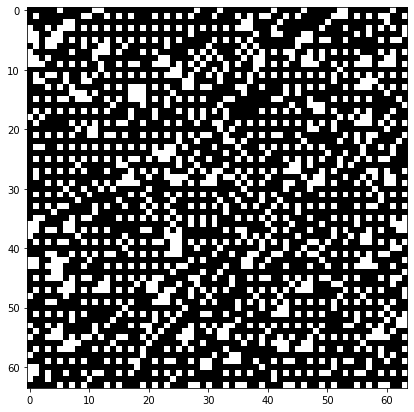
\includegraphics[width=0.6\linewidth]{img/dense.png}
  \caption{Macierz gęsta (0.5) przed reorderingiem}
\end{figure}

\begin{figure}[H]
    \captionsetup{justification=centering}
    \centering
  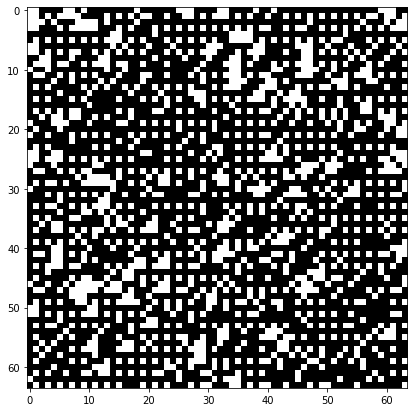
\includegraphics[width=0.6\linewidth]{img/dense_reorder.png}
  \caption{Macierz gęsta (0.5) po reorderingu}
\end{figure}

\begin{figure}[H]
    \captionsetup{justification=centering}
    \centering
  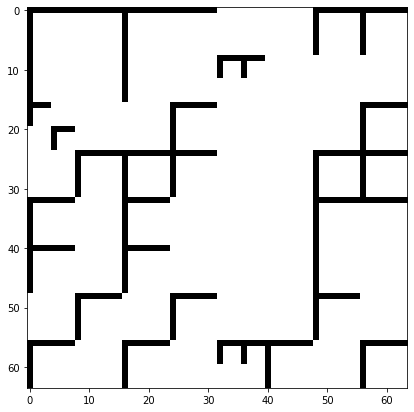
\includegraphics[width=0.6\linewidth]{img/sparse.png}
  \caption{Macierz rzadka (0.01) przed reorderingiem}
\end{figure}

\begin{figure}[H]
    \captionsetup{justification=centering}
    \centering
  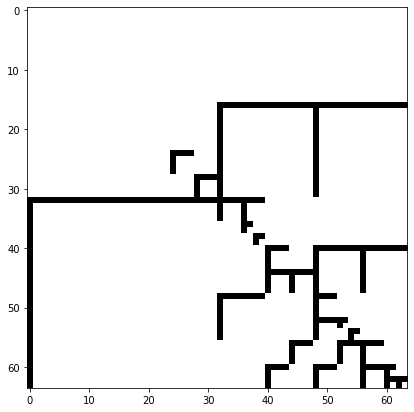
\includegraphics[width=0.6\linewidth]{img/sparse_reorder.png}
  \caption{Macierz rzadka (0.01) po reorderingu}
\end{figure}


\section{Wnioseki}
Widzimy, że dla macierzy gęstych stosowanie reorderingu mija się z celem i nie jest efektywne.
Z kolei podczas używania macierzy rzadkich, możemy uzyskać znaczą optymalizację.
Im rzadsza macierz tym lepsze rezultaty daje reordering.

\end{document}
